\documentclass[10pt]{article}
\usepackage[sc]{mathpazo}
\usepackage{commands}
\hypersetup{colorlinks = true}
\let\oldphi\phi 
\let\phi\varphi 
\let\varphi\oldphi



\begin{document}
\begin{tcolorbox}
  \begin{center}
  \begin{Large}
    \textbf{The Oxford Solid State Basics Textbook Excerices and UBC PHYS 474 Homework Problems} \\
    \vspace{5pt}
  \end{Large}
  \begin{large}
        Tobias Faehndrich \\
\vspace{5pt}
    \emph{This document was last edited on \today}
  \end{large}
  \end{center}
\end{tcolorbox}

\begin{center}
  \textbf{Introduction:}

Homework problems for PHYS 474 which are mainly pulled from Steven Simon's "Oxford Solid State Basics" textbook. If any errors are found, feel free to email me at \href{mailto:tobias.faehndrich@gmail.com}{tobias.faehndrich@gmail.com}.

\end{center}
\addtocontents{toc}{\protect\hypertarget{toc}{}}
\tableofcontents

\newpage
\section[About Condensed Matter Physics]{\hyperlink{toc}{About Condensed Matter Physics}}



\newpage
\section[Specific Heat of Solids - Boltzmann, Einstein, and Debye]{\hyperlink{toc}{Specific Heat of Solids - Boltzmann, Einstein, and Debye}}



\subsection{Einstein Solid (2.1)}

\begin{enumerate}[label=(\alph*)]
    \item \textit{Classical Einstein (or “Boltzmann”) Solid:}

    Consider a three-dimensional simple harmonic oscillator with mass $m$ and spring constant $k$ (i.e., the mass is attracted to the origin with the same spring constant in all three directions). The Hamiltonian is given in the usual way by
    \[
    H = \frac{\vb{p}^2}{2m} + \frac{1}{2} k \vb{x}^2
    \]
    
    \begin{itemize}
        \item Calculate the classical partition function:
        \[
        Z = \int \frac{\dd{\vb{p}}}{(2\pi \hbar)^3} \int \dd{\vb{x}} \, e^{-\beta H(\vb{p}, \vb{x})}
        \]

        Note: in this exercise $\vb{p}$ and $\vb{x}$ are thee-dimensional vectors.

        \divider
        
        We can rewrite that original integral for the partition function then as
        \[
        Z = \recip{(2\pi \hbar)^3} \int \dd{\vb{p}} \int \dd{\vb{x}} \, \e^{-\beta H(\vb{p}, \vb{x})}
        \]

        
        \[
        Z = \recip{(2\pi \hbar)^3} \int \dd{\vb{p}} \int \dd{\vb{x}} \, \e^{-\beta \paren*{ \frac{\vb{p}^2}{2m} + \frac{1}{2} k \vb{x}^2}}
        \]

        \[
        Z = \recip{(2\pi \hbar)^3} \int \dd{\vb{p}} \int \dd{\vb{x}} \, \brackets*{ \e^{-\beta \paren*{\frac{1}{2} k \vb{x}^2}} + \e^{-\beta \frac{\vb{p}^2}{2m}}}
        \]

        \[
        Z = \recip{(2\pi \hbar)^3} \int \e^{-\frac{\beta}{2m} \vb{p}^2} 
        \dd{\vb{p}} \int \e^{-\frac{\beta k}{2} \vb{x}^2} \dd{\vb{x}}
        \]
        

        Using the given \textbf{hint:} You will need to express the vector squares $\mathbf{p}$ and $\mathbf{x}$ in terms of their components. We can safely assume that $\langle p_x^2 \rangle = \langle p_y^2 \rangle = \langle p_z^2 \rangle$ (and similarly for their squared displacements). Note that for some variable $x$:
        \[
        \int_{-\infty}^{\infty} \e^{-\alpha x^2} dx = \sqrt{\frac{\pi}{\alpha}}
        \]

        
        \[ Z = \recip{(2\pi \hbar)^3} \paren*{\sqrt{\frac{2 \pi m}{\beta}}}^3 \paren*{\sqrt{\frac{2 \pi}{\beta k }}}^3\]

        \[ Z = \brackets*{\frac{\sqrt{m}}{\hbar \beta \sqrt{k}}}^3\]

        where $\omega = \sqrt{\frac{k}{m}}$ so that we get

        \[ \boxed{Z = (\omega \hbar \beta)^{-3}}\]

        \item Using the partition function, calculate the heat capacity $3k_B$.

        \divider
        
        Recall the useful formula we derived in class that relates the average internal energy to the partition function.

        \begin{itemize}
            \item From lecture 2's Thermodynamics refresher we saw that

        \begin{itemize}
            \item The probability of finding a system, S, that is in thermal equilibrium with a reservoir, R, at some temperature, T, in a given energy state, $E_i$, 
            \begin{center}
            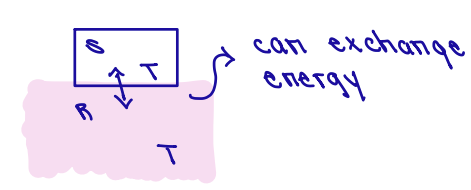
\includegraphics[width = 0.25\textwidth]{Images/Lecture2-thermo.png}
            \end{center}
            
            is given by 
    
            \[
            \mathbb{P}(E_i) \propto \mathrm{e}^{-\beta E_i}
            \]
    
            where $\beta = \frac{1}{k_B T}$ with units of $\left[ \frac{1}{\text{energy}}\right]$
    
            Note that the exponential term is the Boltzmann distribution
    
            \item We can use the \textbf{partition function (Z)} to normalize our probabilities.
    
            i.e. so that we get $\sum_i \mathbb{P} (E_i) = 1$
    
            \[ \mathbb{P} (E_i) = \frac{\mathrm{e}^{-\beta E_i}}{\mathrm{e}^{-\beta E_1} + \mathrm{e}^{-\beta E_2} + \dots } = \frac{\mathrm{e}^{-\beta E_i}}{Z}\]
    
            where $Z = \sum_i \mathrm{e}^{-\beta E_i}$
    
            \item The \textbf{expecation value (or thermal average)} for a given quantity is the sum of the possible values weighted by their normalized probabilities.
    
            \[ \angles{x} = \sum_i x_i \Prob (E_i) = \sum_i x_i \paren*{\frac{\e^{-\beta E_i}}{Z}} = \recip{Z} \sum_i x_i \e^{-\beta E_i} \]
    
            where $ Z = \sum_i \e^{-\beta E_i} $
    
            \item Taking the \textbf{derivative of the partition function with respect to $\beta$} we uncover a useful trick.
    
            \[ \dv{Z}{\beta} = \sum_i \paren*{-E_i } \, \e^{-\beta E_i} \]
    
            Divide by $-Z$ and we get 
    
            \[ \frac{-1}{Z} \dv{Z}{\beta} = \recip{Z} \sum E_i \e^{-\beta E_i} = \angles{E}\]
    
            Thus we get the equation that relates the average internal energy to the partition function.
    
            \[ \angles{E} = \frac{-1}{Z} \dv{Z}{\beta}\]
        \end{itemize}

        which is useful because we want to calculate $C = \dv{\angles{E}}{T}$

        \[ Z = \omega^{-3} \hbar^{-3} \beta^{-3}\]

        \[ \dv{Z}{\beta} = -3 \omega^{-3} \hbar^{-3} \beta^{-4} \]

        \[ \angles{E} = \frac{-3 \omega^{-3} \hbar^{-3} \beta^{-4}}{- \omega^{-3} \hbar^{-3} \beta^{-3}} = \frac{3}{\beta} \]

        where again $\beta = \frac{1}{k_B T}$

        \[ \angles{E} = 3 k_B T \]

        so now we can calculate the heat capacity as

        \[ C = \dv{\angles{E}}{T}\]

        \[ \boxed{C = 3 k_B}\]

        \end{itemize}
        
        
        \item Conclude that if you can consider a solid to consist of $N$ atoms all in harmonic wells, then the heat capacity should be $3Nk_B = 3R$, in agreement with the law of Dulong and Petit.

        \divider 
        The energy of a solid that consists of $N$ atoms all in harmonic wells (each with energy $H = \frac{\vb{p}^2}{2m} + \frac{1}{2} k \vb{x}^2$) can be represented by a sum

        \[
        H = \sum_i^{N} H_i
        \]

        So the partition function can be written as
    
        \[
        Z = \int \frac{\dd{\vb{p}}}{(2\pi \hbar)^3} \int \dd{\vb{x}} \, e^{-\beta \sum_i^{N} H_i(\vb{p}, \vb{x})}
        \]

        Then expanded as
        \[
        Z = \prod_i^{N} \int \frac{\dd{\vb{p}}}{(2\pi \hbar)^3} \int \dd{\vb{x}} \, \brackets*{e^{-\beta H_i(\vb{p}, \vb{x})}} = \brackets*{\int \frac{\dd{\vb{p}}}{(2\pi \hbar)^3} \int \dd{\vb{x}} \, \brackets*{e^{-\beta H_i(\vb{p}, \vb{x})}}}^N
        \]

        Using the result of the integral before 

        \[ Z = (\omega \hbar \beta)^{-3 N} \]

        \[ \dv{Z}{\beta}  = -3N  \omega^{-3N} \hbar^{-3N} \beta^{-3N-1} \]

        \[ \angles{E} = \frac{-1}{Z} \dv{Z}{\beta} = \frac{3N \omega^{-3N} \hbar^{-3N}  \beta^{-3N-1}}{\omega^{-3 N} \hbar^{-3 N} \beta^{-3 N}}\]

        \[ \angles{E} = \frac{3 N}{\beta} = 3 N k_B T \]

        \[ C = \dv{\angles{E}}{T}\]

        \[ \boxed{C = 3 N k_B = 3 R}\]
        
    \end{itemize}   

    \item \textit{Quantum Einstein Solid:}

    Now consider the same Hamiltonian quantum-mechanically.
    \begin{itemize}
        \item Calculate the quantum partition function:
        \[
        Z = \sum_j e^{-\beta E_j}
        \]
        where the sum over $j$ is a sum over all eigenstates.
        
        \divider
        
        Recall from lecture 3 that in Einstein's model for specific heat he improved upon Boltzmann's model by treating each atom as a quantum mechanical simple harmonic oscillator, still being held in place in each spatial direction by a spring that vibrates at a frequency, $\omega$.

        \[ E_n = \hbar \omega \paren*{n + \frac{1}{2}}\]
    
        where $\omega$ is the frequency of the spring, and n is the quantum number. Note that in this model the atoms are still not connected to each other. The given hint suggest that we can perform this entire calculation for 1-dimension before generalizing to 3-dimensions so first in 1D:

        \[
        Z = \sum_n \e^{-\beta \hbar \omega \paren*{n + \frac{1}{2}}}
        \]

        From lecture 3 we got the hint to use the relations:

        \[ \sum_n x^n = \recip{1-x} \quad \text{for } \abs{x} < 1\]

        so here we can let $x = e^{- \beta \hbar \omega}$ to get the desired form:

        \[ Z = \sum_n x^{(n+ \frac{1}{2})} = x^{\frac{1}{2}} \sum_n x^n \]

        and since $\abs{e^{-\beta \hbar \omega}} < 1 $:

        \[ Z = x^{\frac{1}{2}} \cdot \frac{1}{1-x}\]

        \[ Z = \brackets*{\e^{- \beta \hbar \omega}}^{\frac{1}{2}} \cdot \frac{1}{1-\brackets*{\e^{- \beta \hbar \omega}}}\]

        \[ Z = \frac{\e^{- \frac{\beta \hbar \omega}{2}}}{1- \e^{-\beta \hbar \omega}}\]

        another lecture 3 hint was to use the relation:

        \[ \sinh{(x)} = \frac{\e^x - \e^{-x}}{2}\]

        so

        \[ \frac{1}{\sinh{(x)}} = \frac{2}{\e^x - \e^{-x}} \]

        so

        \[ Z = \frac{\e^{ \frac{\beta \hbar \omega}{2}}}{\e^{\frac{\beta \hbar \omega}{2}}} \cdot  \frac{\e^{- \frac{\beta \hbar \omega}{2}}}{1- \e^{-\beta \hbar \omega}} = \frac{1}{\e^{ \frac{\beta \hbar \omega}{2}} - \e^{- \frac{\beta \hbar \omega}{2}}}\]


        \[ \boxed{ Z = \frac{1}{2 \sinh{\paren*{\frac{\beta \hbar \omega}{2}}}} }\]

        \item Explain the relationship with Bose statistics.
        
        \divider

        From the hint given, we will calculate the expectation value of the energy $\avg{E}$ before explaining the relationship with Bose statistics.

        \[ \avg{E} = \frac{-1}{Z} \dv{Z}{\beta} \]

        Using wolfram alpha we get 

        \[
        \frac{d}{d\beta} \left( \frac{1}{2 \sinh\left( \frac{\beta \hbar \omega}{2} \right)} \right)
        = -\frac{1}{4} \hbar \omega \coth\left( \frac{\beta \hbar \omega}{2} \right) \csch\left( \frac{\beta \hbar \omega}{2} \right)
        \]

        \[ \avg{E} = - 2 \sinh{\paren*{\frac{\beta \hbar \omega}{2}}} \cdot -\frac{1}{4} \hbar \omega \coth\left( \frac{\beta \hbar \omega}{2} \right) \csch\left( \frac{\beta \hbar \omega}{2} \right)\]

        Again using WA to simplify:

        \[
        \avg{E} = \frac{1}{2} \hbar \omega \coth\left( \frac{\beta \hbar \omega}{2} \right)
        \]

        where 

        \[
        \coth{(x)} = \frac{e^{-x} + e^{x}}{e^{x} - e^{-x}}
        \]

        Now we want to find some relationship between this result and Bose statistics so we can recall from lecture 2 that both \textbf{Bose-Einstein} and \textbf{Fermi-Dirac Statistics} describe the energy distribution of quantum particles

        \begin{itemize}
            \item BE: photons, Cooper pairs, He$^4$, atomic vibrations (phonons)

            \item The Bose occupation factor $n_B$ gives the number of bosonic particles occupying a given energy state at a given temperature.

            As $T \xrightarrow{} 0$, all particles occupy the ground state.
    
            \begin{center}
                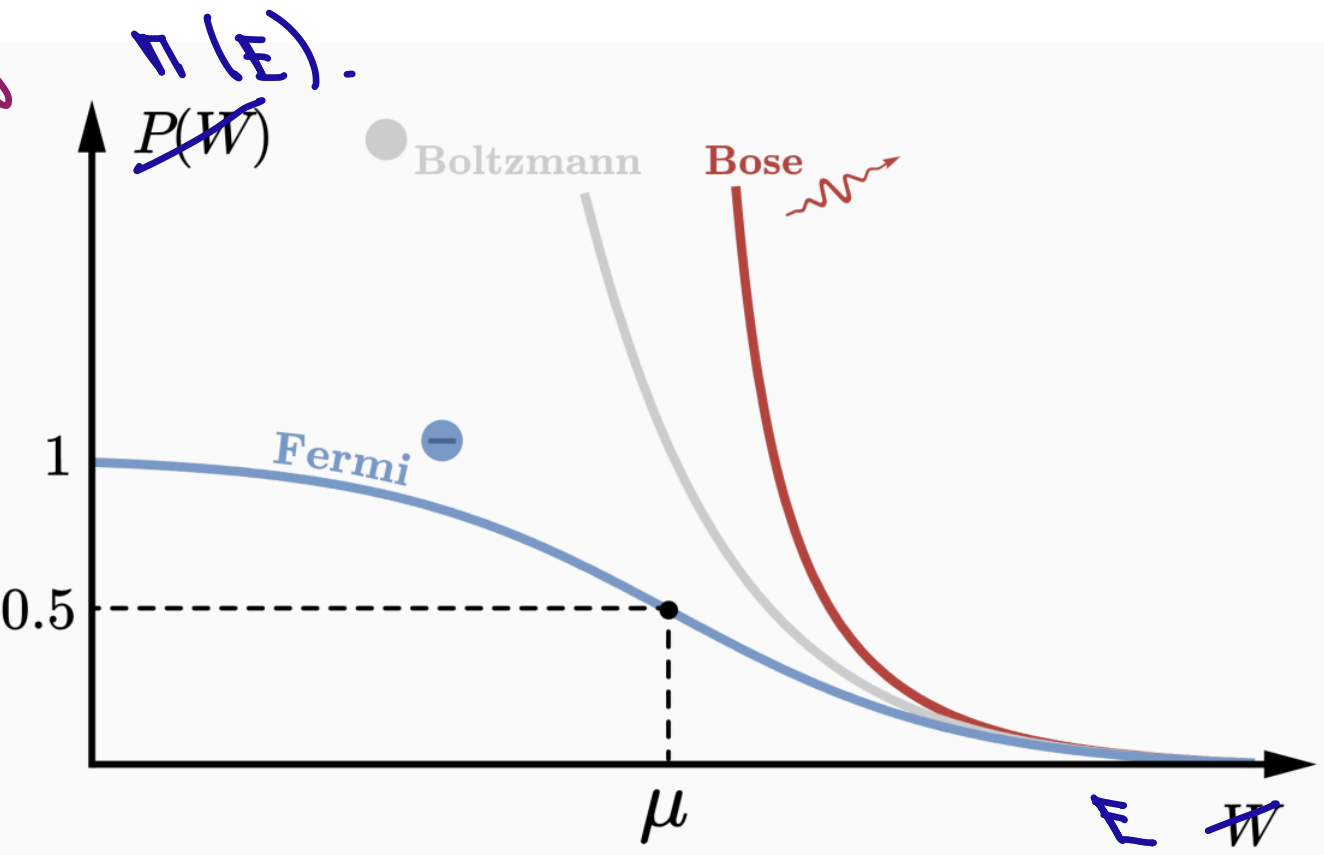
\includegraphics[width = 0.4 \textwidth]{Images/ground-state-distribution-bose-fermi.png}
            \end{center}
    
            \[ n_B = \recip{\e^{(E-\mu) \beta} -1}\]
    
            \vspace{1px}
            
            \item where in the high T limit looks identical to Boltzmann distribution.
    
            \item as $T \rightarrow 0$, $\beta \rightarrow \infty$ and only the lowest E state ($E \approx \mu$) is occupied
    
            \item and $\mu$ is the chemical potential (energy cost to add a particle to the system)
        \end{itemize}

        so now we can go back to our expectation value for the energy and see if we can massage the form to relate it the bose statistics:

        \[
        \coth{(x)} = \frac{e^x}{e^x} \cdot \frac{e^{-x} + e^{x}}{e^{x} - e^{-x}} = \paren*{1 + e^{2x}} \cdot \frac{1}{e^{2x}- 1}
        \]

        \[
        \avg{E} = \frac{1}{2} \hbar \omega \paren*{1 + e^{\beta \hbar \omega}} \cdot \frac{1}{e^{\beta \hbar \omega}- 1}
        \]

        and letting $\hbar \omega = E-\mu $:

        \[
        \avg{E} = \frac{1}{2} \hbar \omega n_B \paren*{1 + e^{\beta \hbar \omega}}
        \]

        \[ \avg{E} = \hbar \omega \paren*{\frac{n_B}{2} + \frac{\e^{\beta \hbar \omega}}{2(e^{\beta \hbar \omega}-1)}}\]

        From WA

        \[ \frac{e^x}{e^x -1} = \frac{1}{e^x - 1} + 1 \]

        \[ \avg{E} = \hbar \omega \paren*{\frac{n_B}{2} + \frac{n_B}{2} + \frac{1}{2}} \]
        
        \[\boxed{ \avg{E} = \hbar \omega \paren*{ n_B + \frac{1}{2}}}\]

        Which is the same form as the quantum mechanical energy for a simple harmonic oscillator but here the Bose occupation facter $n_B$ is in the place of the quantum number n.

        \[ n_B = \recip{\e^{(E-\mu) \beta} -1}\]

        \[ \beta = \frac{1}{kT}\]

        For small $T \rightarrow 0$ we get $\beta \rightarrow \infty$ and $n_B \rightarrow 0$

        \[ \avg{E} \approx \frac{\hbar \omega }{2}\]

        which is the energy of a classical simple harmonic oscillator.

        For large $T \rightarrow \infty$ we would have $\beta \rightarrow 0 $, and recall that for $\e^x$ with small x we can approximate it as $1+x$. Which would give

        \[ \avg{E} \approx \hbar \omega \paren*{\frac{1}{\hbar \omega \beta} + \frac{1}{2}}\]

        \[ \avg{E} \approx k_B T + \frac{1}{2} \hbar \omega \]

        with T term being dominate

        \[ \avg{E} \approx k_B T\]
        
        \item Find an expression for the heat capacity.
        
        \divider

        The quantum partition function in 3D would be:

        \[
        Z_{3D} = \sum_{n_x, n_y, n_z} \e^{-\beta \hbar \omega \paren*{n_x +n_y + n_y + \frac{3}{2}}} = \sum_{n_x, n_y, n_z} \e^{-\beta \hbar \omega n_x} \e^{-\beta \hbar \omega n_y} \e^{-\beta \hbar \omega n_z} \e^{-\beta \hbar \omega \frac{3}{2}}
        \]

        result from before then to the third power:

        \[ Z_{3D} = \brackets*{\frac{1}{2 \sinh{\paren*{\frac{\beta \hbar \omega}{2}}}}}^3 \]

        \[ \avg{E_{3D}} = \frac{-1}{Z_{3D}} \dv{Z_{3D}}{\beta} \]

        Using the chain rule

        \[ \avg{E}_{3D} = \frac{-1}{\brackets*{\frac{1}{2 \sinh{\paren*{\frac{\beta \hbar \omega}{2}}}}}^3} \cdot 3 \brackets*{\frac{1}{2 \sinh{\paren*{\frac{\beta \hbar \omega}{2}}}}}^2 \dv{Z_{1D}}{\beta} \]

        \[ \avg{E_{3D}} = \frac{-3}{Z_{1D}} \dv{Z_{1D}}{\beta} \]

        \[ \avg{E_{3D}} = 3 \avg{E_{1D}} =  3\hbar \omega \paren*{ n_B + \frac{1}{2}} \]

        \[ n_B = \recip{\e^{(E-\mu) \beta} -1}\]
        
        \[ \avg{E_{3D}} = 3 \hbar \omega \paren*{\recip{\e^{\frac{\hbar \omega}{k_B T}} -1} + \frac{1}{2}} \]

        
        Now follow the suggestions from lecture:

        \[ C = \dv{\avg{E_{3D}}}{T} \]

        \[ C = \frac{3 \hbar^2 \omega^2 \e^{\frac{\hbar \omega}{k_BT}}}{k_B T^2 \paren*{\e^{\frac{\hbar \omega }{k_B T}}-1}^2}\]

        Equivalent to the form given as the solution in class:
        
        \[ \boxed{ C = 3 k_B (\beta \hbar \omega)^2 \cdot \frac{\e^{\beta \hbar \omega}}{(\e^{\beta \hbar \omega} -1)^2} }\]

        Note that this expression depends on temperature! 

        
        \item Show that the high-temperature limit agrees with the law of Dulong and Petit.
        
        \divider

        We must make an approximation here, so we can let the exponential term in the denominator use $\e^x \approx 1 + x $ for small $x$.

        \[ C \approx  \frac{3 \hbar^2 \omega^2 \e^{\frac{\hbar \omega}{k_BT}}}{k_B T^2 \paren*{1 + \frac{\hbar \omega }{k_B T}-1}^2}\]

        \[ C \approx  \frac{3 \cancel{\hbar^2 \omega^2} \e^{\frac{\hbar \omega}{k_BT}}}{\cancel{k_B} \cancel{T^2} \frac{\cancel{\hbar^2 \omega^2} }{k_B^{\cancel{2}} \cancel{T^2}}}\]

        When T is large the exponential term on the top goes to 1, leaving us with 

        \[ \boxed{ C \approx 3 k_B }\]
        
        
        \item Sketch the heat capacity as a function of temperature. (See also Exercise 2.7 for more on the same topic.)
        
        \divider

        Skipping final part.
    \end{itemize}

    \end{enumerate}

\subsection*{2. Additional Question}
Some \textbf{solids} have heat capacities that are larger or smaller than 3R at room temperature. Based on what we’ve discussed in class so far (or from reading the textbook), describe a physical scenario that could lead to:
\begin{enumerate}[label=(\alph*)]
    \item $C<3R$ at room temperature

    \divider

    Diamond was the example given in class. The spring constant of the oscillator here in diamond is larger and thus takes a much larger temperature to unfreeze these vibrations.
    
    \item $C > 3R$ at room temperature. (Hint: reading through Chapter 2 of SSB should give you some ideas).

    \divider

    Solids that have more degrees of freedom than those defined by vibrations alone. The textbook briefly mentions ``In magnetic materials there may be still other contributions to the heat capacity reflecting the energy stored in magnetic degrees of freedom". Once you add other terms for these dof then you can expect the heat capacity to be slightly larger.

    
\end{enumerate}


\subsection{Debye Theory I (2.2) -- \textbf{only part (a)}}

\begin{enumerate}[label=(\alph*)]
    \item State the assumptions of the Debye model of heat capacity of a solid.

    \divider

    \begin{itemize}
        \item solids are not just a bunch of atoms at the bottom of a harmonic oscillator but that the atoms would get pushed around by each other and create vibrational waves, i.e. sound waves

        \item these sound waves would be quantized similar to how Planck showed with light

        \item $\omega = v \abs{\vb{k}}$
        \item 3 polarizations oscillation modes. Longitudinal and Transverse (unlike light which is only transverse).
        \item To fix the high temp problem, Debye later adds the max Debye freq cutoff which forces the total number of sound wave modes  to be 3N 

        \item \textbf{Optional Assumptions}
        \begin{itemize}
            \item velocity is the same in transverse and longitudinal directions (not true but assumption can be worked in for not that much more effort).
            \item period boundary conditions for solid. can apply other BCs but this type is the easiest to work.
        \end{itemize}
        
    \end{itemize}

    

    This question asks that you derive the Debye expression for the heat capacity in three dimensions, i.e. the steps found in SSB pgs. 11-14. The point is to be able to justify each step to yourself conceptually (i.e. the significance of the cut-off frequency, what the density of states means).
    
    % \item Derive the Debye heat capacity as a function of temperature (you will have to leave the final result in terms of an integral that cannot be done analytically).

    % \divider

    
    % \item From the final result, obtain the high- and low-temperature limits of the heat capacity analytically.

    % \divider
    
    % \item You may find the following integral to be useful:
    % \[
    % \int_0^\infty \frac{x^3}{e^x - 1} \, dx = \sum_{n=1}^{\infty} \int_0^\infty x^3 e^{-nx} dx = 6 \sum_{n=1}^\infty \frac{1}{n^4} = \frac{\pi^4}{15}
    % \]
    
    % By integrating by parts, this can also be written as:
    % \[
    % \int_0^\infty \frac{x^4 e^x}{(e^x - 1)^2} dx = \frac{4 \pi^4}{15}
    % \]

    % \divider
    
    % \item The following table gives the heat capacity $C$ for potassium iodide as a function of temperature:

    % \begin{center}
    % \begin{tabular}{cc}
    % \toprule
    % $T\,[\mathrm{K}]$ & $C\,[\mathrm{J\,K^{-1}mol^{-1}}]$ \\
    % \midrule
    % 0.1 & $8.5 \times 10^{-7}$ \\
    % 1.0 & $8.6 \times 10^{-4}$ \\
    % 5 & 0.12 \\
    % 8 & 0.59 \\
    % 10 & 1.1 \\
    % 15 & 2.8 \\
    % 20 & 6.3 \\
    % \bottomrule
    % \end{tabular}
    % \end{center}

    % \divider

    % \item Discuss, with reference to the Debye theory, and make an estimate of the Debye temperature.

    % \divider
    
\end{enumerate}

\subsection{Debye Theory II (2.3)}

Use the Debye approximation to determine the heat capacity of a two-dimensional solid as a function of temperature.

\begin{itemize}
    \item State your assumptions.
    
    \item You will need to leave your answer in terms of an integral that one cannot do analytically.
    
    \item At high $T$, show the heat capacity goes to a constant and find that constant.
    
    \item At low $T$, show that $C_v = K T^n$. Find $n$. Find $K$ in terms of a definite integral.
\end{itemize}

If you are brave, you can try to evaluate the integral, but you will need to leave your result in terms of the Riemann zeta function.

\divider

This question has you re-trace the conceptual steps from 2.2 above to derive relations for a two-dimensional solid. The dimensionality's importance enters into the derivation right away for pages 11-14. 

\[ \sum_k \rightarrow \paren*{\frac{L}{2\pi}}^2 \int \dd{\vb{k}}\]

with the integral here being over all \textbf{two} dimensions of $\vb{k}$-space. Debye's method was that the oscillation modes of a solid were waves with frequencies $\omega(\vb{k}) = v\abs{k}$ with v the sound velocity -- and for each $\vb{k}$ for our question here there should be two possible oscillation modes, one for each of the dimensions here. 

\begin{align}
    \avg{E} &= 2 \sum_{\vb{k}} \hbar \omega (\vb{k}) \paren*{(n_B(\beta \hbar \omega(\vb{k}))} \\
            &= 2 \paren*{\frac{L}{2\pi}}^2 \int \dd{\vb{k}} \hbar \omega (\vb{k})) \paren*{n_B ( \beta \hbar \omega(\vb{k})) + \frac{1}{2}}
\end{align}

By radial symmetry, we can convert the 2D integral to a 1D integral

\[ \int \dd{\vb{k}} \rightarrow 2 \pi \int_0^{\infty} k dk\]

since instead of surface area of the sphere of radius k, we are now looking at the circumference of a circle with radius k.
\[ \avg{E} = 2 \paren*{\frac{L}{2\pi}}^2 2 \pi \int \dd{k} k \hbar \omega (\vb{k}) \paren*{n_B ( \beta \hbar \omega(\vb{k})) + \frac{1}{2}}\]

We also use $k=\omega/v$ and $\dv{k}{\omega} = 1/v$

\[ \avg{E} =  \int 2 \paren*{\frac{L}{2\pi}}^2 2 \pi \frac{1}{v} \dd{\omega} \frac{\omega}{v} \hbar \omega  \paren*{n_B ( \beta \hbar \omega) + \frac{1}{2}}\]

following the grouping in equation (2.4) from the textbook (SSB);

\[ \avg{E} =  \int L^2  \brackets*{\frac{4\pi\omega} {(2\pi)^2v^2 }} \dd{\omega} (\hbar \omega)  \paren*{n_B ( \beta \hbar \omega) + \frac{1}{2}}\]

so we could define a 2D version of the density of states as:

\[ g(\omega) = L^2  \brackets*{\frac{4\pi\omega} {(2\pi)^2v^2 }}\]

we can then skip ahead the the realization that integrating to infinite would lead to problems, so we can make the same guess as Debye, that should be only as many modes as there are degrees of freedom in the system. Thus only integrating to some $\omega_{\text{cutoff}}$ or $\omega_{\text{Debye}}$, so that with this frequency, there are exactly 2N sound wave modes in the system (two dimensions of motion times N particles). We thus define $\omega_{\text{cutoff}}$ via

\[ 2N = \int_{0}^{\omega_{\text{cutoff}}} \dd{\omega} g(\omega) \] 

\[ 2N = \int_{0}^{\omega_{\text{cutoff}}} \dd{\omega} L^2  \brackets*{\frac{4\pi\omega} {(2\pi)^2v^2 }}  = L^2 \frac{4 \pi}{(2 \pi)^2 v^2} \frac{\omega_{\text{cutoff}}^2}{2}\]

As the textbook does, we can let $nL^2 = N$, so that we can replace $L^2$ with $N/n$. Where $n$ is the area density of atoms

\[ 2N = \frac{N}{n} \frac{4 \pi }{(2 \pi)^2 v^2} \frac{\omega_{\text{cutoff}}^2}{2}\]

Solving for

\[ \omega_{\text{cutoff}}^2 = 4 \pi n v^2 = \omega^2_D\]

Where the cutoff frequency is also called the Debye frequency. We can compute the heat capacity from the energy using $C = \pdv{\avg{E}}{T}$

\[ \avg{E} =   L^2  \brackets*{\frac{4\pi \hbar} {(2\pi)^2v^2 }} \int \dd{\omega}   \frac{\omega^2}{\e^{\beta \hbar \omega}-1} +  \text{ T independent constant}\]

\[ C = L^2  \brackets*{\frac{4\pi \hbar} {(2\pi)^2v^2 }} \int \dd{\omega} \pdv{}{T} \brackets*{\frac{\omega^2}{e^\frac{\hbar \omega}{k T}-1}} + 0\]

\[ C = L^2  \brackets*{\frac{4\pi \hbar} {(2\pi)^2v^2 }} \int \dd{\omega} \pdv{}{T} \brackets*{\omega^2 (e^\frac{\hbar \omega}{k T}-1)^{-1}} \]

\[ C = L^2  \brackets*{\frac{4\pi \hbar} {(2\pi)^2v^2 }} \int \dd{\omega} \brackets*{-1 \cdot \omega^2 (e^\frac{\hbar \omega}{k T}-1)^{-2} \e^{\beta \hbar \omega} \cdot -1 \cdot \frac{\hbar \omega}{k T^2}} \]

\[ C = L^2  \brackets*{\frac{4\pi \hbar} {(2\pi)^2v^2 }} \int \dd{\omega} \brackets*{\omega^2     \frac{k_B (\beta \hbar \omega)^2}{\hbar \omega} \frac{\e^{\beta \hbar \omega}}{(e^{\beta \hbar \omega}-1)^{2}}} \]

\[ C = L^2  k_B \beta^2 \hbar^2 \brackets*{\frac{4\pi } {(2\pi)^2v^2 }} \int \dd{\omega} \brackets*{\omega^3 \frac{\e^{\beta \hbar \omega}}{(e^{\beta \hbar \omega}-1)^{2}}} \]

Now we can evaluate the integral from 0 to the 2D Debye frequency:

\[ C = L^2  k_B \beta^2 \hbar^2 \brackets*{\frac{4\pi } {(2\pi)^2v^2 }} \int_0^{\omega_D} \dd{\omega} \brackets*{\omega^3 \frac{\e^{\beta \hbar \omega}}{(e^{\beta \hbar \omega}-1)^{2}}} \]

For large T, $\beta \rightarrow 0$, and so $\e^{\beta \hbar \omega} \rightarrow \beta \hbar \omega + 1$


\[ C = L^2  k_B \beta^2 \hbar^2 \brackets*{\frac{4\pi } {(2\pi)^2v^2 }} \int_0^{\omega_D} \dd{\omega} \brackets*{\omega^3 \frac{\beta \hbar \omega + 1}{( \beta \hbar \omega)^{2}}} \]

\[ C = L^2  k_B \beta^2 \hbar^2 \brackets*{\frac{4\pi } {(2\pi)^2v^2 }} \int_0^{\omega_D} \dd{\omega} \brackets*{\frac{\omega^2}{\beta \hbar}+\frac{\omega}{(\beta \hbar)^2}} \]

\[ C = L^2  k_B \beta^2 \hbar^2 \brackets*{\frac{4\pi } {(2\pi)^2v^2 }} \brackets*{\frac{\omega_D^3}{3 \beta \hbar}+\frac{\omega_D^2}{2(\beta \hbar)^2}} \]

simplified with WA to

\[ C = \frac{k L^2 \omega_D^2 (2 \beta \hbar \omega_D + 3)}{6 \pi v^2}\]

Again $\beta$ is small so we can simplify to:

\[ C =  \frac{k L^2 \omega_D^2 }{2 \pi v^2}\]

Recall $\omega_D^2 = 4 \pi n v^2$ and $L^2 = N/n$


\[ C =  \frac{k N/n 4 \pi n v^2 }{2 \pi v^2}\]

So for the high temperature regime of a solid in 2D:

\[ \boxed{C_{\text{2D, high T}}  \approx  {2 k_B N}}\]


In the low temperature limit, $\beta \rightarrow \infty$ , then $\e^{\beta \hbar \omega} \gg 1$. We also can note that at Low T the debye frequency will seem large comparatively, and so we can approximate the integral as going to infinity.

\[ C = L^2  k_B \beta^2 \hbar^2 \brackets*{\frac{4\pi } {(2\pi)^2v^2 }} \int_0^{\omega_D} \dd{\omega} \brackets*{\omega^3 \frac{\e^{\beta \hbar \omega}}{(e^{\beta \hbar \omega}-1)^{2}}} \]

\[ C \approx  L^2  k_B \beta^2 \hbar^2 \brackets*{\frac{4\pi } {(2\pi)^2v^2 }} \int_0^{\infty} \dd{\omega} \brackets*{\omega^3 \e^{- \beta \hbar \omega}} \]

Variable substitution: $x = \beta \hbar \omega$, $\dv{x}{\omega}=\beta \hbar \quad \Rightarrow \dd{\omega} = \frac{1}{\beta \hbar} \dd{x}$

\[ C \approx  L^2  k_B \beta^2 \hbar^2 \brackets*{\frac{4\pi } {(2\pi)^2v^2 }} \frac{1}{\beta \omega} \frac{1}{\beta^3 \hbar^3} \int_0^{\infty} \dd{x} \brackets*{x^3 \e^{- x}} \]

Where this integral evaluates to 6 using WA:

\[ C \approx  L^2  k_B \beta^2 \hbar^2 \brackets*{\frac{4\pi } {(2\pi)^2v^2 }} \frac{1}{\beta \omega} \frac{1}{\beta^3 \hbar^3} 6 \]

So a bunch of constants with a proportionality to $T^2$ at low temperature:

\[ C \approx  \text{Constants } \cdot \frac{1}{\beta^2} \]


\[ \boxed{C_{\text{2D, Low T}} \sim T^2}\]

\subsection*{5. Mini-Project \#1.}
On the Assignments page on Canvas, you will find a (real) heat capacity data set for a newly discovered material, Nd$_5$Rh$_4$Ge$_{13}$ [real materials can have complicated chemical formulas]. The first column is temperature in units of [K] and the second column is raw (unnormalized) heat capacity in units of [$\mu$J/K]. The sample's mass was measured to be 6.1 mg. In this mini-project, you are going to analyze the data and produce a publication-style figure. Note that you do no not to worry about error analysis for this week.

\begin{enumerate}
    \item Produce a graph of heat capacity vs. temperature, where the heat capacity is normalized in units of [J/mol-K]. Hint: to normalize the data you will need to use the molar mass and the mass of the sample. You can calculate the molar mass using the Lenntech calculator (\url{https://www.lenntech.com/calculators/molecular/molecular-weight-calculator.htm}).

    \divider
    
    \begin{center}
        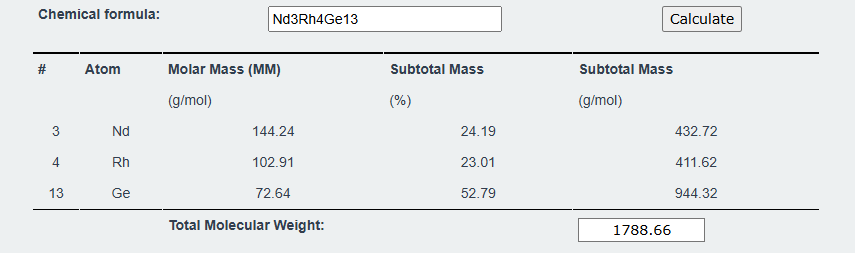
\includegraphics[width = 0.8\linewidth]{Images/molar-mass-hw1.png}
    \end{center}

    Using the molecular weight of 1788.66 g / mol and that the sample has a mass of 6.1 mg.

    \item Add a dashed, labeled horizontal line to your graph at the Dulong-Petit limit. Hint: How many vibrational modes do you expect per formula unit of Nd$_5$Rh$_x$Ge$_{13}$? Count the number of atoms per formula unit!

    \divider 

    In a unit Nd$_5$Rh$_4$Ge$_{13}$ there is 3 + 4 + 13 = 20 atoms, so that in 3D the dulong petit limit will just be $C_{\text{DP}} = 3 \cdot 20 \cdot R$, where $R = 8.314  \text{ J / mol}\cdot K $.

    \item Add a dashed, labeled vertical line to your graph at the Debye temperature $T_{\text{Debye}}$. To calculate $T_{\text{Debye}}$ you can use the relationship for the low-temperature limit of the heat capacity $C = nR \frac{12\pi^4}{5 T_{\text{Debye}}^3} T^3$ where $n$ is the number of atoms per formula unit. In order to accurately estimate the Debye temperature, one should plot C vs T$^3$ for \underline{only} the data below 20 K and fit the data to a straight line. Then, compare the slope of that line to the equation above.
    
    \divider

    \begin{figure}[ht]
    \centering
    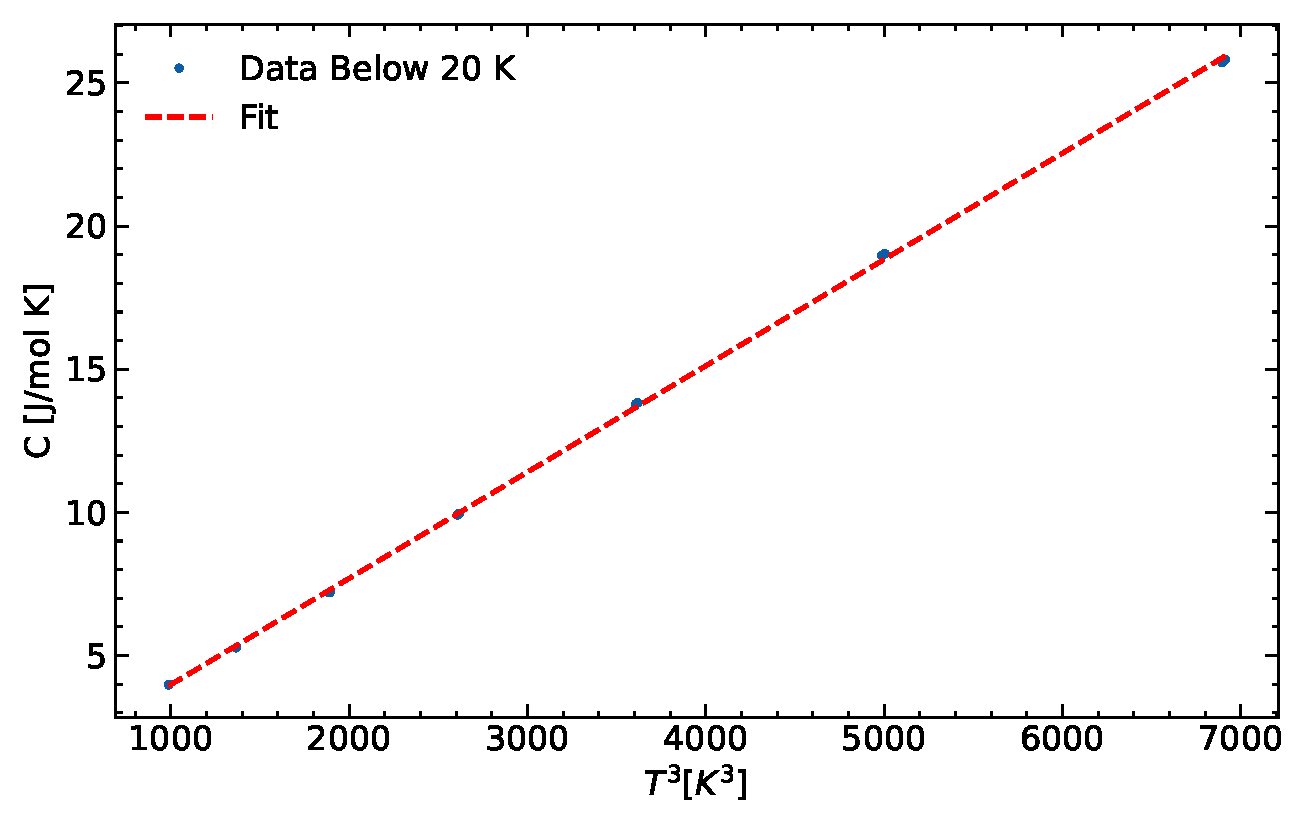
\includegraphics[width=\linewidth]{Images/HW1_c_fit_Debye.eps}
    \caption{Low-temperature ($T < 20\,\mathrm{K}$) heat capacity of Nd$_3$Rh$_4$Ge$_{13}$ plotted as a function of $T^3$. The data exhibits a linear relationship, consistent with the Debye model in the low-temperature limit where $C \propto T^3$. The slope of the best-fit line is used to estimate the Debye temperature $T_{\mathrm{Debye}}$ by comparing to the theoretical expression $C = nR \frac{12\pi^4}{5 T_{\text{Debye}}^3} T^3$.}
    \label{fig:debye_fit}
    \end{figure}

    \begin{figure}[ht]
    \centering
    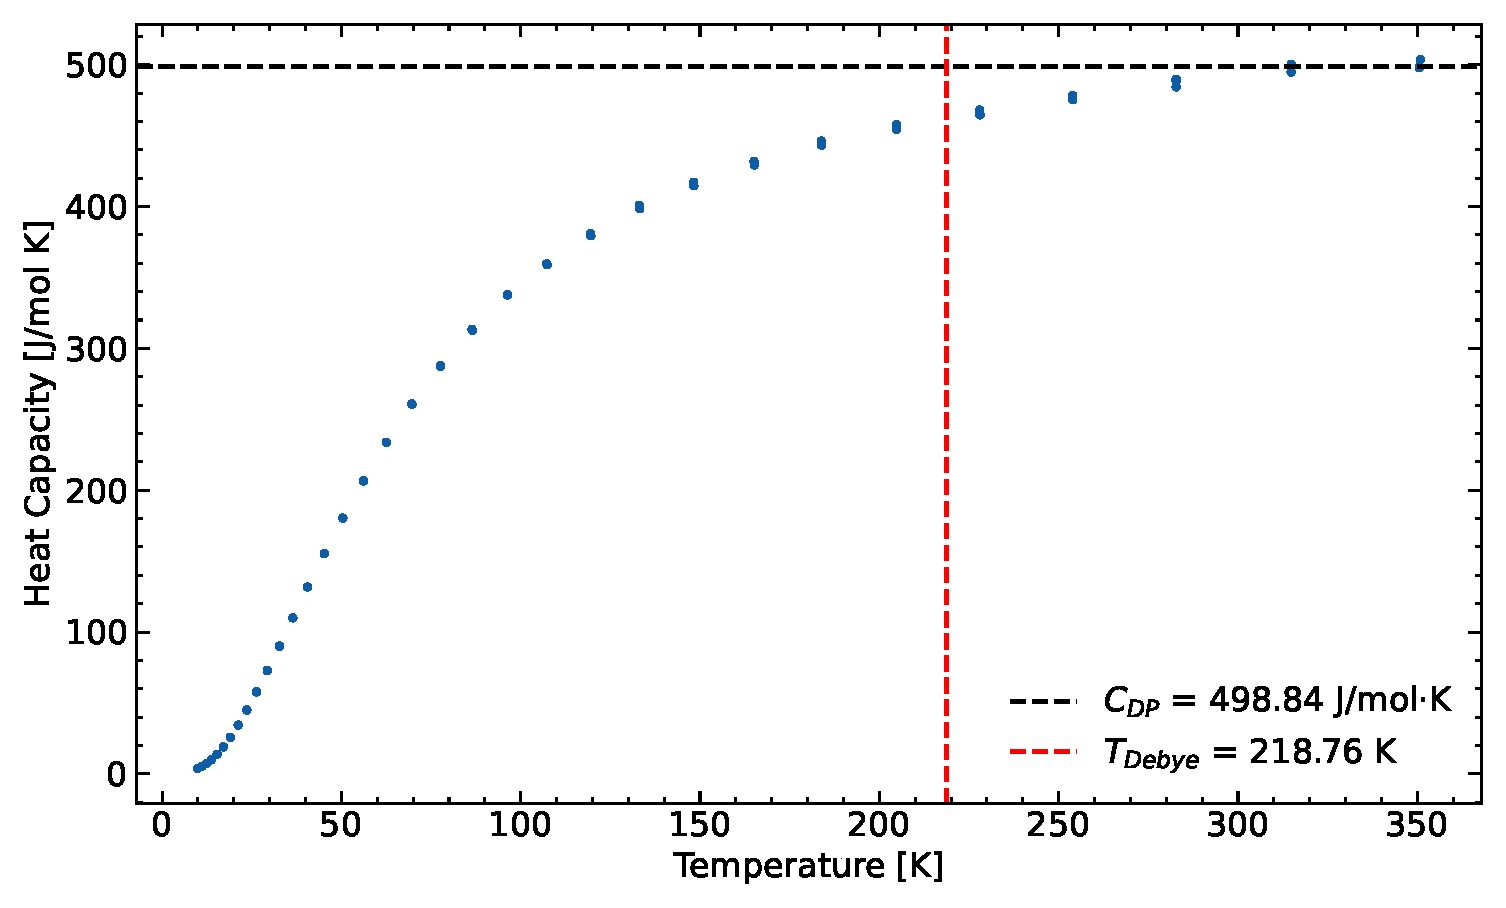
\includegraphics[width= \linewidth]{Images/HW1_c_Debye_Annotated.eps}
    \caption{Heat capacity of Nd$_3$Rh$_4$Ge$_{13}$ as a function of temperature, normalized per mole of sample. The dashed black line marks the Dulong--Petit limit ($C = 3nR$), which represents the high-temperature classical limit of heat capacity. The vertical dashed red line indicates the estimated Debye temperature, obtained by fitting the low-temperature ($T < 20\,\mathrm{K}$) data to the form $C \propto T^3$.}
    \label{fig:debye_annotated}
    \end{figure}


    \item Write a descriptive figure caption for your completed figure. A good figure caption has enough detail that the reader can make sense of what they are looking at (i.e. what is the quantity being plotted, what is the sample that was measured) but should also be succinct. You should draw the reader's attention to key features of interest (i.e. consider the features you labeled in parts (b) and (c)).

    \divider 

    See figure \ref{fig:debye_fit} and figure \ref{fig:debye_annotated}.


\end{enumerate}





\newpage
\section[Drude Theory of Electrons in Metals Sommerfeld Free Electron Theory of Electrons in Metals]{\hyperlink{toc}{Drude Theory of Electrons in Metals Sommerfeld Free Electron Theory of Electrons in Metals}}


\subsection*{3.1 \quad Drude Theory of Transport in Metals}

\begin{enumerate}[label=(\alph*)]
\item Assume a scattering time $\tau$ and use Drude theory to derive an expression for the conductivity of a metal.


\divider 

\begin{itemize}
    \item This is the same derivation from class, so let's consider the derived equation of motion from the Drude model when we have a non-zero electrical field (with $\mathbf{B}$ still 0):
    
    \[ \vec{E} \neq 0, \quad \vec{B} = 0 \]

    Equation of motion:

    \[ \dv{\vec{p}}{t} = -e \vec{E} - \frac{\vec{p}(t)}{\tau} \]

    \item We can now define the conductivity of a metal, $\sigma$, which is the constant of proportionality between the current density $\vec{j}$, and the applied electric field $\vec{E}$.
    
    \begin{center}
        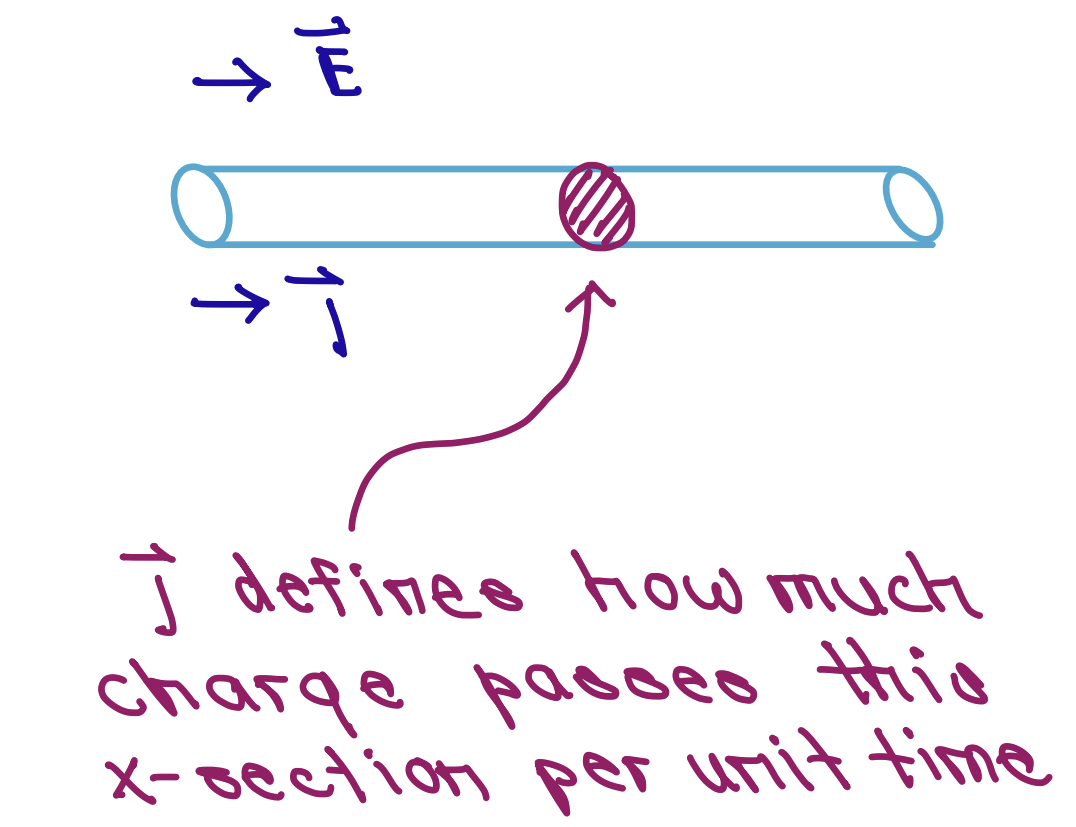
\includegraphics[width = 0.3 \linewidth]{Images/current-density.png}
    \end{center}

    where

    \[\vec{j} = \text{current density} \]
    
    which is the charge per unit time per unit area

    \[ \vec{j} = - n e \vec{v} \]

    where $n$ is the density of electrons   

    \[ \brackets*{e^-/m^3}\brackets*{C/e^-} \brackets*{m/s} = \frac{C}{m^2 \cdot s} \]

    \[ \vec{j} = \frac{e^2 n \tau}{m} \vec{E} \Rightarrow \boxed{\sigma = \frac{e^2 n \tau}{m}} \text{ units } \brackets*{\Omega^{-1} m^{-1}}\]

\end{itemize}


\item Define the resistivity matrix $\underset{\sim}{\rho}$ as 
$\mathbf{E} = \underset{\sim}{\rho}\,\mathbf{j}$. 
Use Drude theory to derive an expression for the matrix 
$\underset{\sim}{\rho}$ for a metal in a magnetic field. 
(You may assume $\mathbf{B}$ parallel to the $\hat{z}$ axis. 
The under-tilde means that the quantity $\rho$ is a matrix.) 
Invert this matrix to obtain an expression for the conductivity matrix 
$\underset{\sim}{\sigma}$.

\divider

\begin{center}
    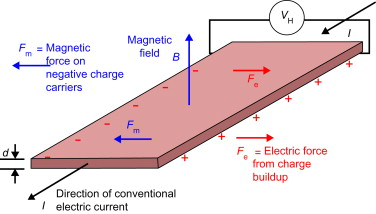
\includegraphics[width = 0.4 \linewidth]{Images/hall-effect.jpg}
\end{center}

For simplicity of typsetting I will use $\rho$ instead of $\underset{\sim}{\rho}$ (and likewise for $sigma$) until the final step.

Recall -- equation of motion derived in lecture 5:

\[ \dv{\vec{p}}{t} = F - \frac{\vec{p}(t)}{\tau} \]

\[ \dv{\vec{p}}{t} = -e \left( \vec{E} + \vec{v} \times \vec{B} \right) - \frac{\vec{p}(t)}{\tau} \]

If we again assume steady state ($\dv{p}{t} = 0$), we get:

\[ 0 = -e \left( \vec{E} + \vec{v} \times \vec{B} \right) - \frac{\vec{p}(t)}{\tau} \]

\[ e \vec{E} = - e \left( \vec{v} \times \vec{B} \right) - \frac{\vec{p}(t)}{\tau}\]

\[ \vec{E} = - \left( \vec{v} \times \vec{B} \right) - \frac{\vec{p}(t)}{e \tau}\]

Recall that $\vec{j} = -ne \vec{v}$ and $\vec{p} = m \vec{v}$. Thus, we can substitute these into the equation as $\vec{p} = \frac{m}{-ne} \vec{j}$ and $\vec{v} = \frac{-1}{ne} \vec{j}$:

\[ \vec{E} = \left( \frac{m}{ne^2 \tau} \right) \vec{j} + \left( \frac{1}{ne} \right) \vec{j} \times \vec{B} \]

where the first term is "longitudinal"  and the second term is off diagonal. Here $\vec{B} = B_z \hat{z}$. We are given the quation:
\[ \vec{B} \parallel \hat{z}, \quad \vec{j} \text{ can be applied along } \hat{x}, \hat{y}, or \hat{z} \]
    
\[ \mathbf{E} = \rho \mathbf{j} \]

We can define a 3 x 3 resistivity matrix for $\undertilde{\rho}$.

\[ \vec{E} = \left( \frac{m}{ne^2 \tau} \right) \begin{pmatrix}
    j_x \\ j_y \\ j_z
\end{pmatrix} + \left(\frac{1}{ne} \right) \begin{pmatrix}
    j_x , j_y , j_z
\end{pmatrix} \times \begin{pmatrix}
    0 \\ 0 \\ B_z
\end{pmatrix} \]

Look at just the cross product we can use the determinant form:

\[ \begin{vmatrix}
    \hat{x} & \hat{y} & \hat{z} \\
    j_x & j_y & j_z \\
    0 & 0 & B_z
\end{vmatrix}  =  j_y B_z \hat{x} - j_x B_z \hat{y} \]


Giving us
\[ \vec{E} = \begin{pmatrix}
\left( \frac{m}{ne^2 \tau} \right) j_x + \left(\frac{B_z}{ne} \right) j_y \\
\left( \frac{m}{ne^2 \tau} \right) j_y - \left(\frac{B_z}{ne} \right) j_x \\
\left( \frac{m}{ne^2 \tau} \right) j_z
\end{pmatrix} \]

Issolating the $\vec{j}$ we can pull out the $\rho$ term.

\[ \vec{E} = \begin{pmatrix}
    \frac{m}{ne^2\tau}& \frac{B}{ne}& 0 \\
    -\frac{B}{ne}&\frac{m}{ne^2\tau}& 0 \\
    0& 0& \frac{m}{ne^2\tau}\\
\end{pmatrix}
\begin{pmatrix}
    j_x \\ j_y \\ j_z
\end{pmatrix}\]

\[ \underset{\sim}{\rho} = \begin{pmatrix}
    \rho_{xx} & \rho_{xy} & 0 \\
    \rho_{yx} & \rho_{yy} & 0 \\
    0 & 0 & \rho_{zz}
    \end{pmatrix} = \begin{pmatrix}
        \frac{m}{ne^2 \tau} & \frac{B}{ne} & 0 \\
        -\frac{B}{ne} & \frac{m}{ne^2 \tau} & 0 \\
        0 & 0 & \frac{m}{ne^2 \tau}
    \end{pmatrix}
 \]

\[ \rho_{xx} = \rho_{yy} = \rho_{zz} = \frac{m}{ne^2 \tau} \]

Hall resistivity:

\[ \boxed{\rho_{xy} = -\rho_{yx} = \frac{B}{ne} }\]

We find that the application of a $\mathbf{B}$ field deflects the electrons causing a measurable potential difference in the orthogonal direction -- this is the Hall effect.

Now taking the inverse of the resistivity we can find the conductivity matrix. Since we have terms along the diagonal, we can split up the problem into a 2x2 inverse and a single element.

\[ A = \begin{pmatrix}
    \rho_{xx} & \rho_{xy} \\ -\rho_{xy} & \rho_{yy}
\end{pmatrix} \]

\[ \det(A) = \rho_{xx} \rho_{yy} + \rho_{xy}^2 \]

\[ A^{-1} = \frac{1}{\det(A)} \begin{bmatrix}
    d & -b \\ -c & a
\end{bmatrix} = \frac{1}{\rho_{xx} \rho_{yy} + \rho_{xy}^2} \begin{bmatrix}
    \rho_{yy} & -\rho_{xy} \\ \rho_{xy} & \rho_{xx}
\end{bmatrix}\]

\[ d = \rho_{zz} \Rightarrow d^{-1} = \rho_{zz}^{-1}\]

Thus, we can write the conductivity matrix as:

\[ \sigma = \rho^{-1} = \begin{pmatrix}
    A^{-1} & 0 \\ 0 & d^{-1}
\end{pmatrix} \]

\[ \sigma = \begin{pmatrix}
    \frac{\rho_{yy}}{\rho_{xx} \rho_{yy} + \rho_{xy}^2} & -\frac{\rho_{xy}}{\rho_{xx} \rho_{yy} + \rho_{xy}^2} & 0 \\ \frac{\rho_{xy}}{\rho_{xx} \rho_{yy} + \rho_{xy}^2} & \frac{\rho_{xx}}{\rho_{xx}\rho_{yy}+\rho_{xy}^2} & 0 \\ 0 & 0 & \frac{1}{\rho_{zz}}
\end{pmatrix} \]

Putting the terms for rho back in:

\[
\sigma = \begin{pmatrix}
    \dfrac{\frac{m}{ne^2\tau}}{\left(\frac{m}{ne^2\tau}\right)^2 + \left(\frac{B}{ne}\right)^2} & -\dfrac{\frac{B}{ne}}{\left(\frac{m}{ne^2\tau}\right)^2 + \left(\frac{B}{ne}\right)^2} & 0 \\
    \dfrac{\frac{B}{ne}}{\left(\frac{m}{ne^2\tau}\right)^2 + \left(\frac{B}{ne}\right)^2} & \dfrac{\frac{m}{ne^2\tau}}{\left(\frac{m}{ne^2\tau}\right)^2 + \left(\frac{B}{ne}\right)^2} & 0 \\
    0 & 0 & \dfrac{ne^2\tau}{m}
\end{pmatrix}
\]



\item Define the Hall coefficient.

    
\[ R_H = \frac{-\rho_{xy}}{|B|} = \frac{-1}{ne} \quad \text{ units } \brackets*{m^3/C}\]

    note: "normal" meteals have a negative $R_H$ (NOT a resistance).

    \begin{center}
        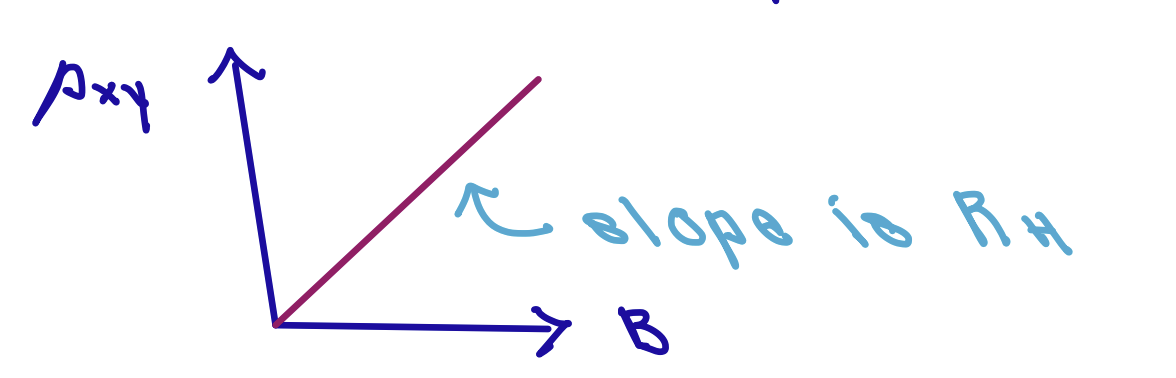
\includegraphics[width = 0.4 \linewidth]{Images/hall-effect-slope.png}
    \end{center}

Some metals have a positive Hall coefficient -- seeming to imply the existence of a positively charged carrier of electrical current. This is forshadowing for later in the course when we will get introduced to the concept of holes in semiconductors.

The Hall coefficient $R_H$ for copper (good metal) is of order 0.1 $mm^3/C$ and its resistivity at RT is of order $10^{-8} \Omega m$. The order of magnitude of the scattering time, $\tau$.
    
    \[ R_H = 0.1 mm^3/C = 10^{-10} m^3/C = \frac{-1}{n e} \]

    \[ \rho = \frac{1}{\sigma} = 10^{-8} \Omega m = \frac{m}{n e^2 \tau} \]

    \[ \tau = \frac{-m R_H}{e^2 \rho} = \frac{-\paren*{10^{-30}\, \text{kg}} \paren*{10^{-10} m^{3}/C}}{\paren*{-10^{-19} C} \paren*{10^{-8} \Omega m}} = 10^{-13} s \]

Average metal $\approx$ 10$^{-14}$ s, so this is reasonable. Scattering time is extraordinarile short. 


\item What properties of metals does Drude theory not explain well?

\item Consider now an applied AC field $\mathbf{E} \sim e^{i \omega t}$ which induces an AC current $\mathbf{j} \sim e^{i \omega t}$. Modify the above calculation (in the presence of a magnetic field) to obtain an expression for the complex AC conductivity matrix $\sigma(\omega)$. For simplicity in this case you may assume that the metal is very clean, meaning that $\tau \to \infty$, and you may assume that $\mathbf{E} \perp \mathbf{B}$. You might again find it convenient to assume $\mathbf{B}$ parallel to the $\hat{z}$ axis. (This exercise might look hard, but if you think about it for a bit, it isn’t really much harder than what you did above!)

\begin{itemize}
    \item At what frequency is there a divergence in the conductivity? What does this divergence mean? (When $\tau$ is finite, the divergence is cut off.)
    \item Explain how could one use this divergence (known as the cyclotron resonance) to measure the mass of the electron. (In fact, in real metals, the measured mass of the electron is generally not equal to the well-known value $m_e = 9.1095 \times 10^{-31}\,\mathrm{kg}$. This is a result of \textit{band structure} in metals, which we will explain in Part VI.)
\end{itemize}

\end{enumerate}


\end{document}
